\documentclass[11pt]{article}
\usepackage[spanish]{babel}
\usepackage[utf8]{inputenc}
\usepackage[T1]{fontenc}
\usepackage{graphicx}
\topmargin=-1.2cm
\textheight=22cm
\textwidth=16cm  
\oddsidemargin=0.45cm  
\setlength{\parindent}{0cm}
\renewcommand{\baselinestretch}{1.1}
\graphicspath{{hola/}}
\title{Actividad 7}
\author{Hinostroza Moya Natalia}
\date{05 de abril de 2017}

\begin{document}
%===============================================================================
% PORTADA
%===============================================================================
\begin{titlepage}
\begin{center}
\includegraphics[scale=0.35]{escudo.png}
\end{center}
\vspace*{0.02in}
\begin{center}

\rmfamily\textbf{\LARGE UNIVERSIDAD DE SONORA}\\
\vspace*{1.02in}
{\Large División de Ciencias Exactas y Naturales}\\
{\Large Departamento de Física}\\

\vspace*{0.99in}
\rule{99mm}{0.1mm}\\
\vspace*{0.4cm}
\textbf{\LARGE Reconstruyendo la señal}\\
\vspace*{0.001in}
\rule{99mm}{0.1mm}

\vspace*{1in}
\normalsize{Autor:}\
\normalsize{Natalia Hinostroza Moya}\\
\vspace*{0.3mm}
\normalsize Profesor:\
\normalsize Carlos Lizárraga Celaya\\
\vspace*{1.5cm}
\normalsize 18 de abril de 2017

\end{center}
\end{titlepage}

%==============================================================================
% DESARROLLO
%==============================================================================
\textbf{\section*{\LARGE Resumen}}
Previamente, en la actividad 6, descompusimos en intervalos de tiempo las mareas de los sitios escogidos por cada uno de los alumnos del curso. Con apoyo de la Tranformada de Fourier Discreta (DFT), extraimos los modos naurales de la marea.\\

Obtenido lo anterior, en esta actividad se pide reconstruir la señal de los valores obtenidos por la DFT, así como encontrar el error relativo de aproximar la señal de la marea. 

\textbf{\section{\LARGE Introducción}}
Con los datos de la actividad pasada utiizaremos la serie de Fourier la cual se utiliza para el estudio de movimientos armónicos. En esta actividad compararemos la serie de Fourier que se obtiene directamente y la que nosotros crearemos con los datos recopilados y estudiados anteriormente.

\textbf{\section{\LARGE Serie de Fourier}}
La serie de Fourier es una serie infinita que converge puntualmente a una funciónperiódica y continua por partes. Esta serie forma parte de una de las herramientas matemáticas básicas de análisis de Fouriel que se empleo para el análicis de funciones periódicas a través de la descomposición de la función en un a suma infinita de funciones sinusoidales simples.\\

Su nombre es en honor al matemático frances Jean-Baptiste Joseph Fourier, que fue quien desarrolló la teoría mientras estudiaba la ecuación de calor. Fue el primero en estudiar las series armónicas.

La serie de Fourier, además de ser una herramienta sumamente útil en la teoría de la matemática abstracta, es muy utilizada en muchas ramas de la ingeniería. Algunas de sus áreas de aplicación incluyen análisis vibratorios, acústica, óptica, procesamiento de imágenes y señales, y comprensión de datos. 

\textbf{\section{\LARGE Mazatlán}}

\begin{verbatim}
def f(t):
 return -900 + (103)*np.sin(np.pi*t/12.9) + (177.3)*np.sin(np.pi*t/12.1) + (79.8)*np.sin(np.pi*t/12) 
+(72.5)*np.sin(np.pi*t/6.3) + (64.6)*np.sin(np.pi*t/6.2) + (342.6)*np.sin(np.pi*t/6.2) + (102.5)*np.sin(np.pi*t/6 ) + (229.8)*np.sin(np.pi*t/5.9) 
#5 + (0.15)*np.sin(np.pi*t/13.16)  + (0.42)*np.sin(np.pi*t/12.2) + (0.08)*np.sin(np.pi*t/6.3) + (0.48)*np.sin(np.pi*t/6.25) + (0.18)*np.sin(np.pi*t/6.0241)

#interpolar la funcion
df[u'WaterLevel'] = df[u'WaterLevel'].astype(float).interpolate(method='spline', order=2)

fig = mplt.gcf()
fig.set_size_inches(12, 7)

mplt.plot(df[u'Hora'], f(df[u'Hora']), c='black', label='Curva construida')
mplt.plot(df[u'Hora'], df[u'WaterLevel'], c='blue', label='Curva original')


mplt.ylabel('Nivel de la marea(mm)')
mplt.xlabel('Hora')
mplt.legend(fancybox=True, shadow=True)
mplt.grid(True)
\end{verbatim}

\begin{center}
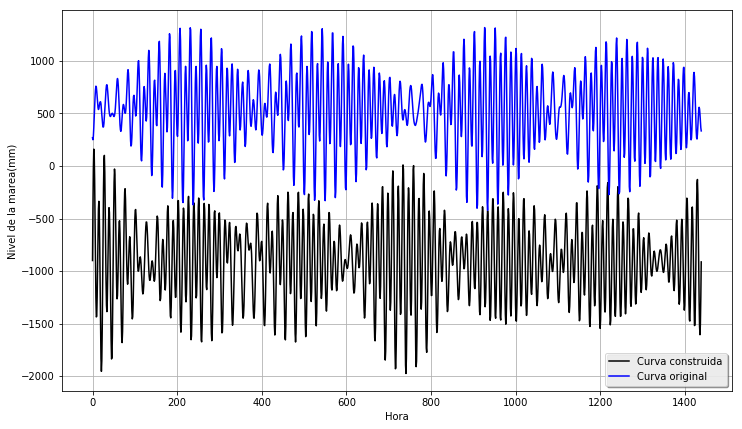
\includegraphics[scale=0.50]{Maz.png}
\end{center}

\textbf{\section{\LARGE San Francisco}}

\begin{verbatim}
def f(t):
 return 3.5 + (0.43)*np.sin(np.pi*t/12.9) + (1)*np.sin(np.pi*t/12) + (0.32)*np.sin(np.pi*t/6.3) + (1.98)*np.sin(np.pi*t/6.2) +(0.35)*np.sin(np.pi*t/6)


#interpolar la funcion
df[u'WaterLevel'] = df[u'WaterLevel'].astype(float).interpolate(method='spline', order=2)

fig = mplt.gcf()
fig.set_size_inches(12, 7)

mplt.plot(df[u'Hora'], f(df[u'Hora']), c='black', label='Curva construida')
mplt.plot(df[u'Hora']+175, df[u'WaterLevel'], c='blue', label='Curva original')


mplt.ylabel('Nivel de la marea(m)')
mplt.xlabel('Hora')
mplt.legend(fancybox=True, shadow=True)
mplt.grid(True)
\end{verbatim}


\begin{center}
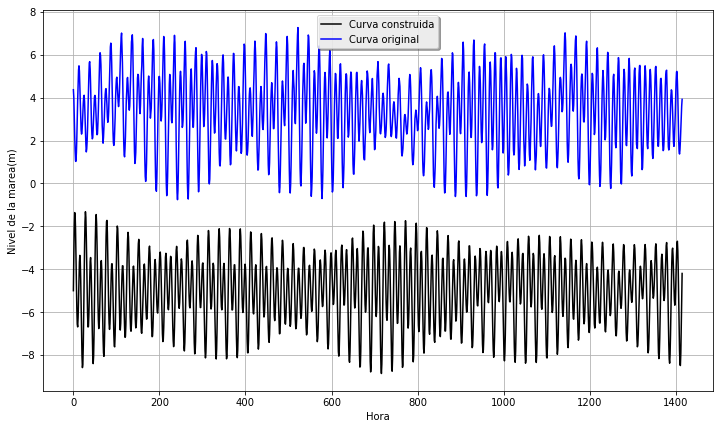
\includegraphics[scale=0.50]{SF.png}
\end{center}

\textbf{\section{\LARGE Conclusión}}
La curva original y la curva construida con los datos que había acomodado no son iguales, pero se puede notar la similitud entre ellas. Otra cosa que puede notarse a simple vista es que están desfasadas, no logré acomodarlas para que quedarán en fase. 
\end{document}




